Verbindung initiieren

FA-C \ref{c-session} %FA-C 33 Websocket Verbindung
FA-KI \ref{ki-session} %FA-KI 39 Websocket Verbindung

Verbindung halten

FA-S \ref{s-clientconnection} %FA-S 4 Client Verbindung
FA-S \ref{s-websockets} %FA-S 19 Websockets
FA-C \ref{c-session} %FA-C 33 Websocket Verbindung
FA-KI \ref{ki-session} %FA-KI 39 Websocket Verbindung

Verbindung wieder aufbauen

FA-S \ref{s-clientconnection} %FA-S 4 Client Verbindung
FA-C \ref{c-persistentsession} %FA-C 34 Persistente Session

Verbindung trennen

FA-S \ref{s-timeout} %FA-S 6 Client Timeout

JSON-Codierung

FA-S \ref{s-json-encoding} %FA-S 17 JSON Encoding
FA-S \ref{s-json-decoding} %FA-S 18 JSON Decoding
FA-C \ref{c-session} %FA-C 33 Websocket Verbindung
FA-KI \ref{ki-session} %FA-KI 39 Websocket Verbindung

Registrieren des Client-Typs

FA-C \ref{c-join-human} %FA-C 24 Registrieren als menschlicher Spieler
FA-KI \ref{ki-register} %FA-KI 40 Registrieren als KI

\begin{figure}
  \centering
  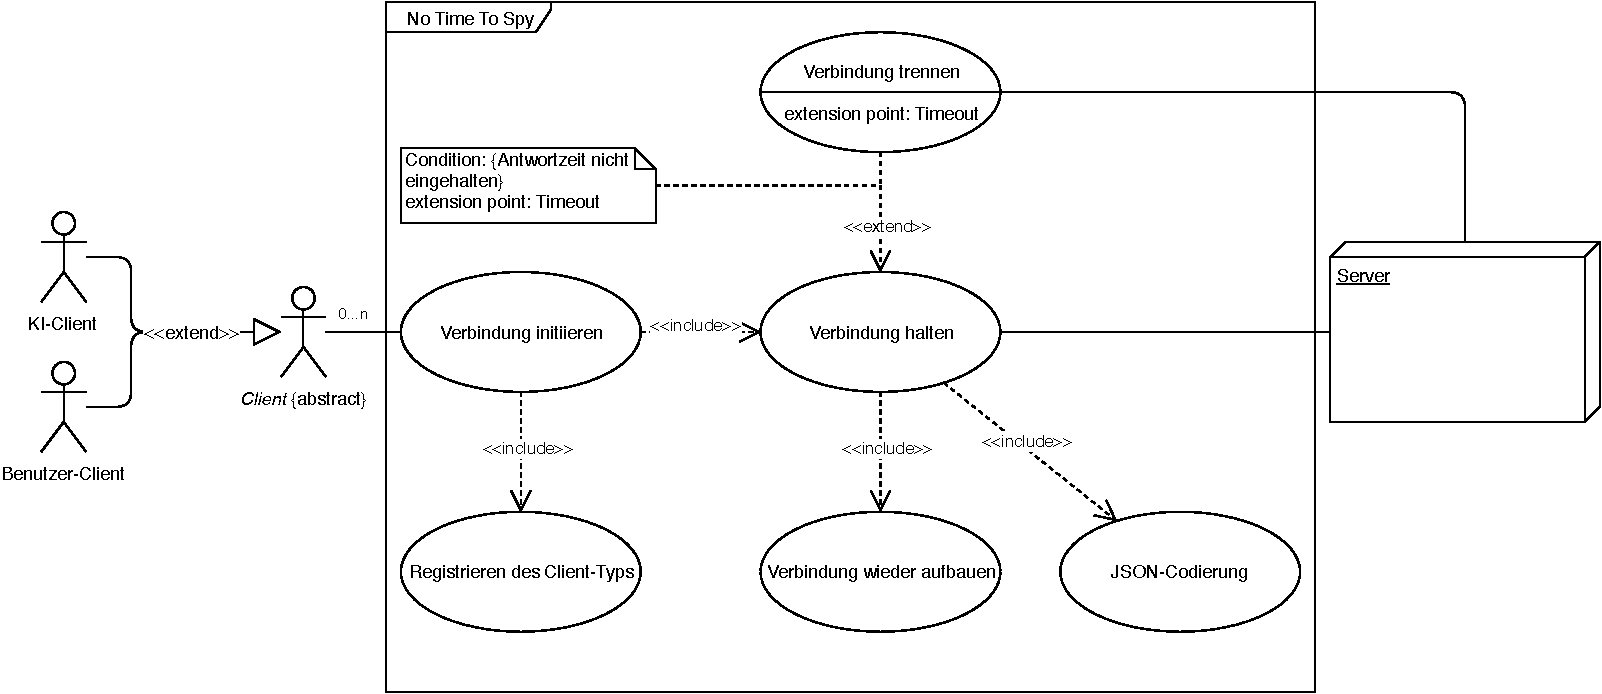
\includegraphics[width=\textwidth]{Meilenstein02/use_case_network.pdf}
  \caption{Anwendungsfälle Netzwerkverbindungsmanagement}
\end{figure}